\section{Routing Proxies}
\label{sec-proxy}



In this section, we first propose {\em routing  proxies} and {\em deterministic routing areas} (\dras) to capture the idea of representatives and the set of
nodes being represented, respectively. We then give an analysis of the properties of  \dras and their routing proxies, and show that they indeed hold the desired properties of representatives that we have discussed in Section~\ref{sec-intro}.
We finally show how to answer shortest path and distance queries using routing proxies.

%We consider a graph $G(V, E, w)$.






\eat{
\begin{figure}
\centering
\begin{minipage}[b]{.5\textwidth}
  \centering
  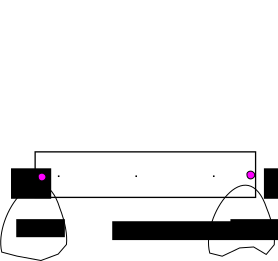
\includegraphics[scale=0.45]{./rep-landmarks.eps}
  %\vspace{-1ex}
  \caption{Using proxies for landmarks}
  \label{fig-angent-landmarks}
\end{minipage}
\begin{minipage}[b]{.24\textwidth}
  \centering
  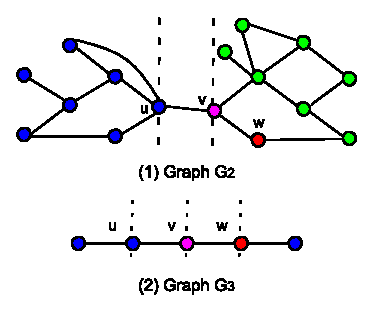
\includegraphics[scale=0.65]{./extended-proxies.eps}
  %\vspace{-1ex}
  \caption{Example proxies and \dras}
  \label{fig-proxies}
\end{minipage}%
\vspace{-4ex}
\end{figure}
}

\subsection{Routing Proxies and Deterministic Routing Areas}
\label{subsec-proxy-def}

We first present the notions of routing proxies and their deterministic routing areas.

\stitle{Proxies}. Given a node $u$ in graph $G(V, E)$, we say that $u$ is a {\em routing proxy} (or simply {\em proxy}) of a set of nodes, denoted by $A_{u}$, if and only if:

\sstab(1) node $u\in A_{u}$ is reachable to any node of $A_u$ in $G$,

\sstab(2) all neighbors of any node $v\in A_u\setminus \{u\}$ are in $A_u$,  and

\sstab(3) the size $|A_u|$ of $A_u$ is equal to or less than $c\cdot\lfloor\sqrt{|V|}\rfloor$, where $c$ is a small constant number, such as $2$ or $3$.


Here condition (1) guarantees the connectivity of subgraph $G[A_u]$,  condition (2) implies that not all neighbors of proxy $u$ are necessarily in $A_u$;
and condition (3), referred to as {\em size restriction}, limits the size of $A_u$ of proxy $u$.
Intuitively, one simply checks the graph by removing $u$ from $G$ and its newly created
\ccs , and a proxy of $u$ is a union of such \ccs whose total number of nodes is at most $c\cdot\lfloor\sqrt{|V|}\rfloor - 1$.




\stitle{Deterministic routing areas}. A node $u$ may be a proxy of multiple sets of nodes $A^1_u, \ldots, A^k_u$, and
we denote as $A^{+}_u$ the union of all the sets of nodes whose proxy is $u$ , \ie  $A^{+}_u$ = $A^1_u$ $\cup\ldots\cup$ $A^k_u$.

We refer to the {\em subgraph} $G[A^+_u]$ as a deterministic routing area (\dra) of proxy $u$.

Intuitively, \dra $G[A^+_u]$ is a {\em maximal} connected subgraph, union of a set of \ccs, that connects to the rest of graph $G$ through proxy $u$ only.
That is, for any node $v$ in $G[A^+_u]$ and any node $v$ in the rest of graph $G$, $u$ must appear on the shortest path $\path(v, v')$.

\stitle{Maximal proxies}.  We say that a proxy $u$ is {\em maximal} if there exist no other proxies $u'$ such that $u'\ne u$ and $A^+_{u} \subset A^+_{u'}$.

\stitle{Trivial proxies}. We say that a maximal proxy $u$ is {\em trivial} if $A^+_u$ contains itself only, \ie $A^+_{u}$ = $\{u\}$.


\stitle{Equivalent proxies}. We say that two proxies $u$ and $u'$ are {\em equivalent}, denoted by $u\equiv u'$, if $A^+_{u} = A^+_{u'}$.




We next illustrate these notions with an example below.

\begin{figure}
\centering
 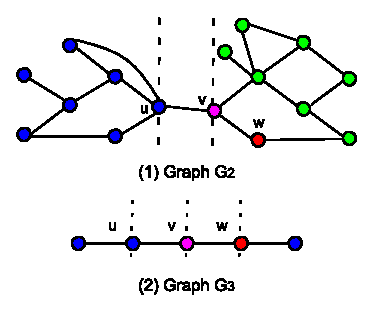
\includegraphics[scale=0.95]{./extended-proxies.eps}
 \vspace{-2ex}
 \caption{Example proxies and \dras}
  \label{fig-proxies}
\vspace{-3ex}
\end{figure}


\vspace{-0.5ex}
\begin{example}
\label{exm-proxies} First consider graph $G_2(V_2, E_2)$ in Fig.~\ref{fig-proxies}, and let $c\cdot\lfloor\sqrt{|V_2|}\rfloor$ =
$2\cdot\lfloor\sqrt{16}\rfloor$ = $8$, where $c = 2$ and $|V_2| = 16$.
\sstab(1) Node $u$ is a proxy, and its \dra is the subgraph in the left hand side of the vertical line across $u$;
\sstab(2) Node $v$ is a proxy, and its \dra is the subgraph in the left hand side of the vertical line across $v$;
\sstab(3) Node $w$ is not a proxy since it can not find a \dra with size less or equal than $8$;
\sstab(4)  Node $v$ is a maximal proxy, while node $u$ is not a maximal proxy since $A^+_u\subset A^+_v$.


We then consider graph $G_3(V_3, E_3)$ in Fig.~\ref{fig-proxies}, and let $c\cdot\lfloor\sqrt{|V_3|}\rfloor$ =
$2\cdot\lfloor\sqrt{5}\rfloor$ = $4$, where $c = 2$ and $|V_3| = 5$.
\sstab(1) Nodes $u, v$ and $w$ are three maximal proxies, whose \dras are all the entire graph $G_3$, and, hence,
\sstab(2) $u, v$ and $w$ are three equivalent proxies.
 \end{example}

\vspace{-1ex}
\stitle{Remark}. As illustrated by the above examples,  a \dra of graph $G(V, E)$ may have a size larger than $c\cdot\lfloor\sqrt{|V|}\rfloor$,
and multiple equivalent proxies.


We next first justify the necessity of introducing the size restriction for proxies.  Otherwise, \dras are simply \ccs, and are mostly useless.


\begin{prop}
\label{prop-proxy-cc} Without the size restriction, any node $u$ in a graph $G$ is a maximal proxy,
and its \dra $G[A^+_u]$ is exactly the connected component (\cc) to which $u$ belongs.
\end{prop}


We then show that proxies and \dras are {\em well defined}.


\begin{prop}
\label{prop-proxy-unique-dra} Any proxy in a graph has a unique \dra.
\end{prop}


\begin{prop}
\label{thm-proxy-disjoint} Given any two distinct proxies $u$ and $u'$, \\
(1) if $u\in A^+_{u'}$, then $A^+_{u}\subseteq A^+_{u'}$, \\
(2) if $u'\in A^+_{u}$, then $A^+_{u'}\subseteq A^+_{u}$,  and \\
(3) $A^+_{u}\cap A^+_{u'}$ = $\emptyset$, otherwise.
\end{prop}


By Proposition~\ref{thm-proxy-disjoint}, it is easy to have the following, which says when maximal proxies are concerned, there exists a unique set of non-overlapping \dras.

\begin{cor}
\label{cor-proxy-disjoint} Given any two maximal proxies $u$ and $u'$, then either $A^+_{u} = A^+_{u'}$ or $A^+_{u}\cap A^+_{u'}$ = $\emptyset$ holds.
\end{cor}


\vspace{-1ex}
\stitle{Remark}. Trivial proxies only represent themselves, and, hence, we are only interested in non-trivial maximal proxies (or simply called proxies) in the sequel.


\subsection{Properties of Proxies and DRAs}
\label{subsec-proxy-properties}

We next give an analysis of proxies and \dras, and show that they indeed hold good properties for answering shortest path and distance queries.
%



Indeed, the size restriction guarantees that the shortest distance computation within a \dra can be evaluated efficiently,
as shown below.


\begin{prop}
\label{pro-proxy-path} Given any two nodes $v, v'$ in the \dra $G[A^+_u]$ of proxy $u$ in graph $G$, \\
(1) the shortest path in $G[A^+_u]$ is exactly the one in the entire graph $G$, and\\
(2) it can be computed in linear time in the size of $G$.
\end{prop}


By Proposition~\ref{pro-proxy-path}, it is easy to derive the following.

\begin{cor}
\label{cor-proxy-distance} Given any two nodes $v, v'$ in the \dra $G[A^+_u]$ of proxy $u$ in graph $G$, \\
(1) the shortest distance $\dist(v, v')$ in $G[A^+_u]$ is exactly the one in the entire graph $G$, and\\
(2) it can be computed in linear time in the size of $G$.
\end{cor}


\begin{prop}
\label{pro-proxy-path-global} Given two nodes $v$ and $u$ with two distinct proxies $x$ and $y$, respectively, in graph $G$, the shortest path from $v$ to $u$ is $\path(v, x)/\path(x, y)/\path(y, u)$.
\end{prop}


Here $\path(v, x)/\path(x, y)/\path(y, u)$ is a path by concatenating paths $\path(v,x)$, $\path(x,y)$ and $\path(y,u)$.
By Proposition~\ref{pro-proxy-path-global}, it is easy to derive the following result.

\begin{cor}
\label{cor-proxy-distance-global} Given two nodes $v$ and $u$ with two distinct proxies $x$ and $y$, respectively, in graph $G$, the shortest distance $\dist(v, u)$ = $\dist(v, x)$ $+$ $\dist(x, y)$  $+$ $\dist(y, u)$.
\end{cor}


Propositions~\ref{pro-proxy-path},~\ref{pro-proxy-path-global} and Corollaries~\ref{cor-proxy-distance},~\ref{cor-proxy-distance-global} guarantee that the shortest paths and distances between the nodes in the \dras of two distinct proxies can be answered in a correct and efficient way.






\subsection{Query Answering with Routing Proxies}
\label{subsec-proxy-query}



\eat{%%%%%%%%
\begin{figure}[tb!]
%\vspace{-1ex}
\begin{center}
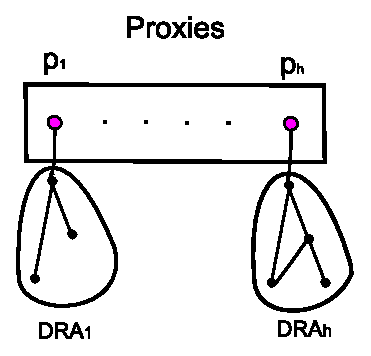
\includegraphics[scale=0.6]{./Proxy-framework.eps}
\end{center}
\vspace{-2ex}
\caption{Framework of using proxies}
\label{fig-angent-landmarks} \vspace{-2ex}
\end{figure}
}%%%%%%%%%%%%EAT

 Based on the above analyses, we present a framework for speeding-up shortest  path and distance query answering, which consists of two modules: {\em preprocessing} and {\em query answering}.
 %The framework for answering queries using proxies and \dras is illustrated in Fig.~\ref{fig-angent-landmarks}, in which each $p_i$ ($i\in[1, h]$) denotes a proxy, and is associated with its \dra.
 We next introduce the details of the framework.

\stitle{1. Preprocessing}. Given graph $G(V, E)$, the preprocessing module executes the following.

\sstab (1) It first computes all \dras and their maximal proxies with algorithm $\compDRAs$ (to be seen shortly in Section~\ref{sec-proxy-algorithms}).

\sstab (2) It then pre-computes and stores all the shortest paths and distances between any node in a \dra and its proxy.


\stitle{2. Query answering}. Given two nodes $s$ and $t$ in graph $G(V, E)$  and the pre-computed information, the query answering module executes the following.


\sstab (1) When nodes $s$ and $t$ belong to the same \dra $G[A^+_u]$ with proxy $u$ such that $A^+_u$ = $A^1_u\cup\ldots A^h_u$.

If $s$ and $t$ further fall into the same $A^i_u$ ($i\in[1,h]$), then it invokes the Dijkstra's algorithm on the subgraph $G[A^i_u]$ to compute the shortest path and distance between $s$ and $t$. Otherwise, it simply returns $\path(s, u)/\path(u, t)$ or $\dist(s, u)$ + $\dist(u, t)$, in constant time.

\sstab (2)  When $s$ and $t$ belong to two \dras $G[A^+_{u_s}]$ and $G[A^+_{u_t}]$ with proxies $u_s$ and $u_t$, respectively.

Observe that $\path(s, t)$ = $\path(s, u_s)/\path(u_s, u_t)/$ $\path(u_t, t)$ and $\dist(s, t)$ = $\dist(s, u_s)$ + $\dist(u_s, u_t)$ + $\dist(u_t, t)$, in which $\path(s, u_s)$, $\path(u_t, t)$, $\dist(s, u_s)$ and $\dist(u_t, t)$ are already known. Hence, it simply invokes an algorithm (\eg bidirectional Dijkstra~\cite{LubyR89}, \arcflag \cite{MohringSSWW05}, \ch~\cite{GeisbergerSSD08}, \tnr~\cite{bast2014route}) for computing $\path(u_s, u_t)$.
Similarly, the shortest distance $\dist(s, t)$ can be computed.

\stitle{Remarks}.
(1) To support shortest distance queries, for each node in a \dra, we store its corresponding proxy and the distance to the proxy. To support shortest path queries, we further keep the shortest paths from each proxy to all nodes in its \dra. Thus, we need $O(d)$ extra space to store the routing information to answer shortest path and distance queries, where $d$ is the total number of nodes in all \dras.

\sstab (2) Let $G'$ be the reduced subgraph of $G$ by removing all the nodes in \dras, but keeping their proxies, from graph $G$. It is easy to see that the main computation cost is reduced from $G$ to $G'$. As shown in the experimental study (Section~\ref{sec-expt}), on average about 1/3 nodes of a graph are captured by non-trivial proxies and their \dras, \ie $d$ is about $|V|/3$. That is, graph $G'$ is about 2/3 size of graph $G$, and hence our data reduction technique could reduce graph sizes and speed up shortest path and distance computations.
